\documentclass[10pt,tgadventor, onlymath]{beamer}

\usepackage{graphicx,amsmath,amssymb,tikz,psfrag,neuralnetwork, stackengine,array, multirow, fontawesome}

\input defs.tex
\graphicspath{ {./figures/} }

%% formatting

\mode<presentation>
{
\usetheme{default}
\usecolortheme{seahorse}
}
\setbeamertemplate{navigation symbols}{}
\usecolortheme[rgb={0.03,0.28,0.59}]{structure}
\setbeamertemplate{itemize subitem}{--}
\setbeamertemplate{frametitle} {
	\begin{center}
	  {\large\bf \insertframetitle}
	\end{center}
}


\usetikzlibrary{shapes,arrows}
\usetikzlibrary{positioning}
\tikzstyle{block} = [rectangle, draw, fill=blue!20, 
    text width=5em, text centered, rounded corners, minimum height=4em]
\tikzstyle{line} = [draw, -latex']

%% begin presentation

\title{\large \bfseries Power Allocation in Heterogeneous Networks for Base Stations with Multiple Antennas}

\author{Peter Hartig \\ \and Supervisor: Prof. Laura  Cottatellucci
}

\date{\today}

\begin{document}

\frame{
\thispagestyle{empty}
\titlepage
}

\section{Project Goals}

\begin{frame}
\frametitle{Objectives}
\begin{enumerate}
\setlength\itemsep{2em}
\item Find a Nash Equilibrium between all players.
\begin{itemize}
\item Preferably a "social optimal" Nash Equilibrium.
\end{itemize}
\item Minimize the resources required to reach Nash Equilibrium.
\end{enumerate}
%\pause
\begin{center}
		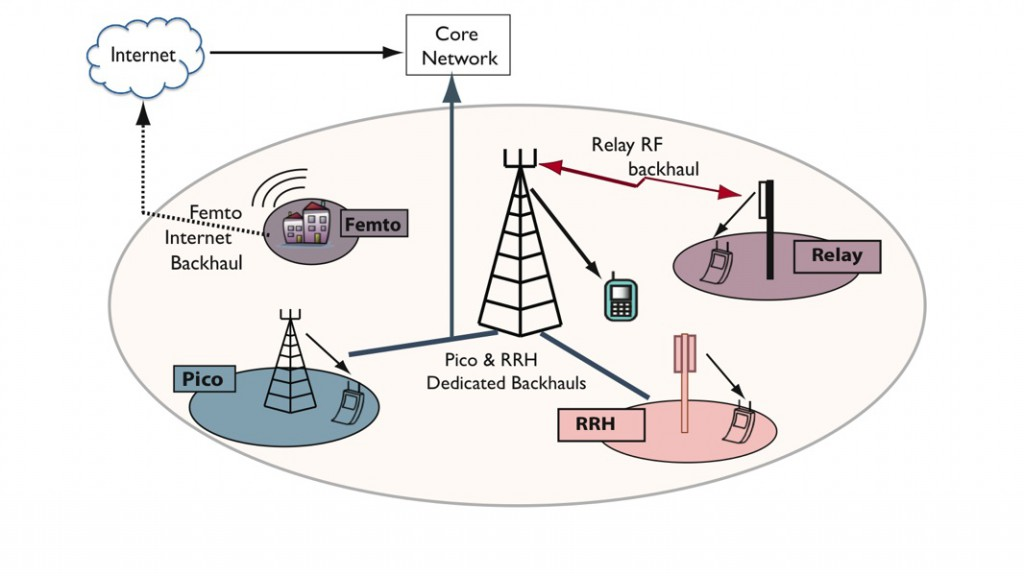
\includegraphics[scale=.2]{het_net}
\end{center}
\end{frame}
\begin{frame}
\frametitle{Key Tools}
\begin{enumerate}
\setlength\itemsep{2em}

\item 
Potential Games 
\begin{itemize}
\item
Games with many players becomes a central optimization problem
\end{itemize}
\item 
N-Person Concave Games
\begin{itemize}
\item
Ensures solution is optimal
\item
Solve the game using convex optimization
\end{itemize}
\item 
Distributed Optimization
\begin{itemize}
\item
Reducing the network overhead needed to reach a solution
\end{itemize}
\end{enumerate}
\end{frame}

\begin{frame}
  \centering \Large
  \emph{Thank You.}
  \\
	\bigskip
    \centering \Large
  \emph{Questions or Comments?}
\end{frame}

\end{document}
